\documentclass[main.tex]{subfiles}
\ifxetex\else
\onlyinsubfile{\usepackage{CJKutf8}}
\fi
\begin{document}
\ifxetex\else\begin{CJK*}{UTF8}{song}\fi

\chapter{准备工作}
%% my chapter 1 content
%\onlyinsubfile{this only appears if chapter1.tex is compiled (not when main.tex is compiled)}
%\notinsubfile{this only appears if main.tex is compiled (not when chapter1.tex is compiled)}
%% more of my chapter 1 content
%%
\section{树莓派介绍}

\par
树莓派 (Raspberry Pi,简写 RPI)是一台卡片计算机,它由英国的树莓派基金会开发,目的是以低价硬件及自由软件促进计算机基础教育,培养孩子们在电子和编程方面的兴趣。从 2012年开始,发布了 1A、 1B、 1B\-+、 Zero、 2B、 3B以及最新的 4B等版,价格在 5-35美元之间。为了增加系统的“可玩性”,树莓派对外引出了几十个引脚,用户可以在电路级别与其他第三方系统连接,从而扩展了系统的功能。正是树莓派这种开放的硬件设计,它在电子爱好者、学生和教师中掀起了一阵 DIY的风暴,通过树莓派与传统的硬件结合,创造了很多有趣且有用的项目。例如,它与无人机结合,用于无人机的控制;与家电结合,形成智能家居系统;通过外接屏幕和按钮,模拟传统的电子游戏机。不仅如此,作为一台功能完整的计算机,它也可以作为 web服务器、文件服务器或者媒体播放器,甚至可以用几十上百台树莓派构建计算机群集。

\par
在软件方面,也遵循了同样的开放设计.树莓派基金会提供了 raspbian,一个基于 Debian的 Linux发行版。官方提供稳定、持续更新的软件平台,是树莓派成功的关键因素之一。

\par
尽管树莓派拥有无限的应用前景,本文并不关注树莓派的应用。我们想把树莓派当作一台普通的计算机,学习运行于 ARM架构上的操作系统。如今操作系统的开发,一般都是在虚拟机上面进行。尽管虚拟机是开发操作系统最高效的平台,但是基于真实的物理机器来开发操作系统会带来不同的体验。树莓派具有物理机器的所有组件,而且它价格便宜、体积小,很适合于学习操作系统内核的设计和开发。由于历史的原因,英特尔的 x86设计相当复杂,初学的门槛比较高。相比之下, ARM架构的发展时间短,指令集相对简单,容易上手,而且树莓派采用了 SoC,单个芯片上集成了 CPU、内存、 GPU以及很多外设控制器,不存在各种兼容性问题。

\section{开发环境}

\subsection{硬件材料}
\begin{itemize}
\item 树莓派:本文采用 1B版做测试,也适用于 1B+版和 zero版,但尚未在 RPI2之后的版本上测试过。该版本树莓派采用博通 (Broad\-com)的 BCM\-2835作为中央处理器,架构上属于 ARMv6的 ARM\-1176\-JZF-S,只有一个核心。

\item USB转串口小板和2根杜邦线:相比于显示器的输出,串口是最容易接收树莓派输出的接口。目前大部分计算机没有串口(也称为 RS232、 UART或 COM口),而配置了多个 USB接口,因此需要一个 USB转串口的小板,如图\ref{figure:1-1}所示。连接方法是将树莓派与小板的 TxD与 RxD对接,如图\ref{figure:1-1}所示。如果你用 1B+版本及其以后的树莓派,它提供了 40个引脚,其中前 26个与 B+之前的版本是兼容的,所以串口的连接方法仍然如图所示。

\begin{figure}[htp]
\centering
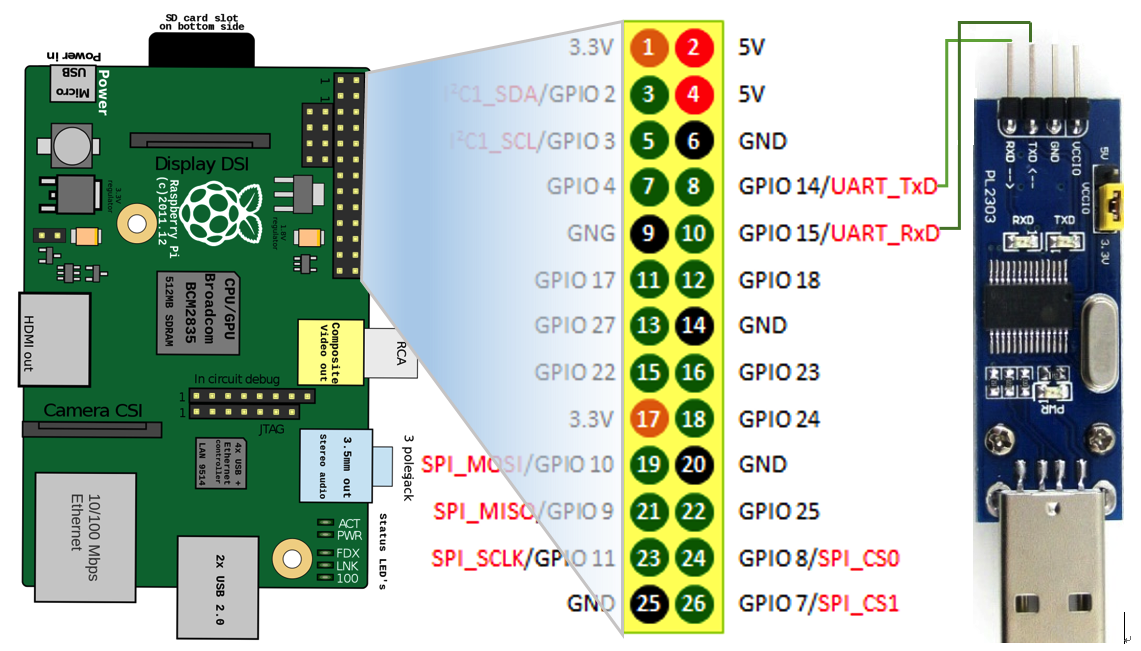
\includegraphics[scale=0.2]{figures/1-1.png}
\caption{树莓派串口连接示意图}
\label{figure:1-1}
\end{figure}

\item 一张 (Micro)SD存储卡及其读卡器。

\item 另外,开发过程中需要频繁给树莓派加电、断电,建议购买一根带开关的 USB电源线,既提高了开发效率,也可以避免频繁拔插USB接口对其造成损害。
\end{itemize}

\subsection{软件环境}
\begin{itemize}
\item 首先,把 SD卡格式化成 FAT32文件系统,然后从 \htmladdnormallink{GitHub}{https://github.com/raspberrypi/firmware/}下载 bootcode.bin和 start.elf两个文件并复制到 SD卡的根目录下。 boot\-code.bin和 start.elf是树莓派的引导程序,功能上类似于 IBM-PC上的 BIOS。
\item 从 ARM公司 \htmladdnormallink{官网}{https://developer.arm.com/tools-and-software/open-source-software/developer-tools/gnu-toolchain/gnu-rm}下载 GNU工具链,解压缩后把 arm-\-none-\-eabi/bin加入到路径 PATH中。
\item 在开发过程中需要用到 GNU make。如果你在 Windows中做开发,可以去 \htmladdnormallink{这里}{https://github.com/mbuilov/gnumake-windows}下载编译好的版本。
\item 准备一个查看串口输出的工具。在 Windows中,可以使用 \htmladdnormallink{PuTTY}{https://www.putty.org}; Unix\-/\-Linux中用 \htmladdnormallink{screen}{https://www.gnu.org/software/screen/}就很好了。

\iffalse
\item \htmladdnormallink{QEMU}{https://www.qemu.org}可以模拟树莓派的部分功能,在后期的开发测试过程中,为了提高开发效率,可以用QEMU来代替,以避免反复的插拔SD卡。在前期开发过程中,不建议用QEMU模拟器。
\fi
\end{itemize}

\clearpage
\ifxetex\else\end{CJK*}\fi
\end{document} 